\documentclass[11pt,a4paper,oneside]{book}
%-- coding: UTF-8 --
\usepackage[UTF8]{ctex}
\usepackage{fontspec}
\defaultfontfeatures{Mapping=tex-text}
\usepackage{xunicode}
\usepackage{xltxtra}
\usepackage{amsmath}
\usepackage{amsfonts}
\usepackage{amssymb}
\usepackage{graphicx}
\usepackage{amsthm}
\usepackage{array}
\usepackage{float}   %{H}
\usepackage{booktabs}  %\toprule[1.5pt]
\setcounter{secnumdepth}{4}
\usepackage{indentfirst} %首行缩进
\usepackage{tcolorbox} %彩色框框
\usepackage{graphicx}  %图片并排
\usepackage{subfigure} %图片并排
\usepackage{graphicx} %插入jpg
\setcounter{secnumdepth}{4}		%增加编号深度
\setcounter{tocdepth}{4}		%增加目录深度
\usepackage{hyperref}     %生成pdf书签
\hypersetup{hidelinks,
	colorlinks=true,
	allcolors=black,
	pdfstartview=Fit
	%,breaklinks=true
}       %去掉目录的红色框框
%===================%插入代码需要的控制
\usepackage{listings}
\usepackage{xcolor}
\setmonofont{Consolas}%字体
\lstset{
	%numbers=left, 
	%qnumberstyle= \tiny, 
	keywordstyle= \color{ blue!70},
	commentstyle= \color{red!50!green!50!blue!50}, 
	frame=shadowbox, % 阴影效果
	rulesepcolor= \color{ red!20!green!20!blue!20} ,
	escapeinside=``,% 英文分号中可写入中文
	breaklines      =   true, 
	basicstyle=\ttfamily 
} 
%===================%
\usepackage[left=2cm,right=2cm,top=2cm,bottom=2cm]{geometry}
\newtheorem{theorem}{定理}
\newtheorem{definition}{定义}
\newtheorem{example}{例}
\pagestyle{plain}%设置页码
\title{\huge 上机课: 时间序列基于R }
\author{zy}
\date{\today}

\begin{document}
\maketitle
\tableofcontents  %目录
\part{时间序列预处理}
\chapter{创建时间序列}
\section{白噪声示例}
\begin{lstlisting}[language=r]
A<-rnorm(n=1000)
wn<-ts(A)
plot(wn)
acf(wn)
\end{lstlisting}
\begin{figure}[H]
	\centering
	\includegraphics[width=\linewidth]{screenshot004}
	\caption{}
	\label{fig:screenshot004}
\end{figure}
\begin{figure}[H]
	\centering
	\includegraphics[width=\linewidth]{screenshot005}
	\caption{}
	\label{fig:screenshot005}
\end{figure}
\begin{lstlisting}[language=r]
> library(forecast)
Registered S3 method overwritten by 'quantmod':
method            from
as.zoo.data.frame zoo 
> Acf(wn)
> Pacf(wn)
> tsdisplay(wn)
\end{lstlisting}
\begin{figure}[H]
	\centering
	\includegraphics[width=\linewidth]{screenshot006}
	\caption{}
	\label{fig:screenshot006}
\end{figure}
\begin{figure}[H]
	\centering
	\includegraphics[width=\linewidth]{screenshot007}
	\caption{}
	\label{fig:screenshot007}
\end{figure}
\begin{figure}[H]
	\centering
	\includegraphics[width=\linewidth]{screenshot008}
	\caption{}
	\label{fig:screenshot008}
\end{figure}


\section{手动录入}
\subsection{矩阵输入}
\begin{lstlisting}[language=r]
> flood.data<-matrix(
+   c(
+     1949 , 1 , 331.12 , 243.96 ,
+     1950 , 2 , 380.44 , 293.90 ,
+     1951 , 3 , 59.63 , 59.63,
+     1952 , 4 , 37.89 , 18.09,
+     1953 , 5 , 103.66 ,72.92,
+     1954 , 6 , 316.67 , 244.57,
+     1955 , 7 , 208.72 , 155.77,
+     1956 , 8 , 288.79 , 255.22),
+   byrow=T, ncol=4,  #按行录入,列数为4
+   dimnames=list(1949:1956,
+                 c("year", "t", "area1", "area2")) #行列命名,前行后列
+ )
> flood.area1 <- ts(flood.data[,"area1"],
+                   frequency=1,  #周期
+                   start=1949)   #起始时间 
> flood.area2 <- ts(flood.data[,"area2"],
+                   frequency=1,
+                   start=1949)
\end{lstlisting}

\subsection{行输入}
\begin{lstlisting}[language=r]
> price<-c(101,82,66,35,31, 7)
> price<-ts(price, start=c(2005,1), frequency=12)
> price
Jan Feb Mar Apr May Jun
2005 101  82  66  35  31   7
\end{lstlisting}
读入半年为单位的数据frequency=2; 季度为单位的数据frcquency=4;
星期为单位的数据frequency=52;日为单位的数据frequency=365.

\subsection{列输入}
\begin{lstlisting}[language=r]
> price<-scan()
1: 12
2: 23
3: 34
4: 56
5: 12
6: 
Read 5 items
> price<-ts(price, start=c(2005,1), frequency=12)
> price
Jan Feb Mar Apr May
2005  12  23  34  56  12
\end{lstlisting}

\section{文件导入}
\begin{lstlisting}[language=r]
> t1.2<-read.csv("E:/5.时间序列/机房eviews&R/时间序列数据/1.2/表1.2.csv")
> t1.2
   年份   CPI
1  1985 109.3
2  1986 106.5
3  1987 107.3
......
21 2005 101.8
22 2006 101.5
23 2007 104.8
> xl<-ts(t1.2$CPI,start=1985)
\end{lstlisting}

\section{文件的导出}
\begin{lstlisting}[language=r]
write.table (x_new, file="E: /R/data/yield.csv", sep="," ,row.names=F)
\end{lstlisting}

\section{产生样本}
\section{生成新序列}
\begin{lstlisting}[language=r]
#子集
z<-subset(bwi.data,Year>1550,select=Beveridge.wheat.price.index)
\end{lstlisting}



\chapter{序列的简单统计量}
\begin{lstlisting}[language=r]
> attributes(CPI)
$tsp
[1] 1985 2007    1

$class
[1] "ts"

> library(psych)
> describe(CPI)
  n   mean   sd median trimmed  mad  min   max range skew kurtosis  se
 23 106.57 7.21  103.9  105.81 5.04 98.6 124.1  25.5 0.95    -0.34 1.5
\end{lstlisting}

%--------------------------------------------------------------%
\chapter{纯随机性检验}\label{cha:01}
拿到一个观察值序列之后,首先是判断它的平稳性.通过平稳性检验,序列可以分为平稳序列和非平稳序列两大类.

对于非平稳序列,由于它不具有二阶矩平稳的性质,所以对它的统计分析要费一些周折,通常要通过进一步的检验,变换和处理,才能确定适当的拟合模型.
\section{纯随机序列的定义}
如果序列值彼此之间没有任何相关性,那就意味着该序列是一个没有记忆的序列,称为纯随机序列.从统计分析的角度,纯随机序列是没有任何分析价值的.
\begin{figure}[H]
	\includegraphics[width=0.85\textwidth]{screenshot009}
	\label{fig:screenshot009}
\end{figure}
\begin{figure}[H]
	\includegraphics[width=0.85\textwidth]{screenshot010}
	\label{fig:screenshot010}
\end{figure}
\begin{lstlisting}[language=r]
> op <- par(no.readonly=TRUE)
> par(op)
> wn<-rnorm(1000)
> wn<-ts(wn)
> plot(wn)
\end{lstlisting}
\begin{figure}[H]
	\includegraphics[width=\textwidth]{screenshot011}
	\label{fig:screenshot011}
\end{figure}
\section{白噪声序列的性质}
\subsection{纯随机性}
$$ \gamma(k)=0,\forall k \neq 0 $$
这说明白噪声序列额各项之间\textbf{没有任何相关关系}.这种没有记忆的序列就是\textbf{纯随机序列}.

如果不是全为0,就说明不是纯随机序列,该序列间隔k期的序列值存在一定程度的相互影响关系,这种相互影响关系系统上称为\textbf{相关信息}.

我们分析的目的就是要想方设法把这种相关信息从观察值序列中提取出来.一旦观察值序列蕴含的相关信息完全提取出来了,那么剩下的残差序列就应该呈现出纯随机序列的性质.所以纯随机性还是判别相关信息提取是否充分的一个判别标准.

\subsection{方差齐性}
$$Var(X_t)=\gamma_0=\sigma^2,\forall t$$
\begin{figure}[H]
	\includegraphics[width=0.85\textwidth]{screenshot012}
	\label{fig:screenshot012}
\end{figure}

\section{纯随机性检验}

\begin{figure}[H]
	\includegraphics[width=0.85\textwidth]{screenshot013}
	\label{fig:screenshot013}
\end{figure}
\begin{lstlisting}[language=r]
> acf(wn)
\end{lstlisting}
\begin{figure}[H]
	\centering
	\includegraphics[width=\textwidth]{screenshot014}
	\label{fig:screenshot014}
\end{figure}
\begin{figure}[H]
	\includegraphics[width=0.85\textwidth]{screenshot015}
	\label{fig:screenshot015}
\end{figure}
\begin{figure}[H]
	\includegraphics[width=0.85\textwidth]{screenshot016}
	\label{fig:screenshot016}
\end{figure}
\subsection{假设条件}
\begin{figure}[H]
	\includegraphics[width=0.85\textwidth]{screenshot017}
	\label{fig:screenshot017}
\end{figure}

\subsection{检验统计量}

\begin{figure}[H]
	\includegraphics[width=0.85\textwidth]{screenshot018}
	\label{fig:screenshot018}
\end{figure}
\begin{figure}[H]
	\includegraphics[width=0.85\textwidth]{screenshot019}
	\label{fig:screenshot019}
\end{figure}
\begin{figure}[H]
	\includegraphics[width=0.85\textwidth]{screenshot020}
	\label{fig:screenshot020}
\end{figure}

计算前面白噪声序列 k=6,k=12的$Q_{LB}$统计量的值,并判断该序列的随机性($ \alpha=0.05 $)
\begin{lstlisting}[language=r]
> Box.test(wn,lag=6)

Box-Pierce test

data:  wn
X-squared = 3.5385, df = 6, p-value = 0.7388

> Box.test(wn,lag=12)

Box-Pierce test

data:  wn
X-squared = 6.7964, df = 12, p-value = 0.8708
\end{lstlisting}
\begin{figure}[H]
	\includegraphics[width=0.85\textwidth]{screenshot021}
	\label{fig:screenshot021}
\end{figure}


\part{平稳时间序列分析}
\chapter{AR models}
\section{建模理论}
\subsection{偏相关系数}
\begin{figure}[H]
	\includegraphics[width=0.85\textwidth]{screenshot064}
	\label{fig:screenshot064}
\end{figure}
\begin{figure}[H]
	\includegraphics[width=0.5\textwidth]{screenshot065}
	\label{fig:screenshot065}
\end{figure}
\subsection{序贯t规则}
由大到小的序贯他规则:

设置最大滞后期$ p_{max} $,令$ \hat{p}=p_{max} $进行估计,然后对最有一个滞后期的系数的显著性进行t检验.

若显著,则停止选定,$ \hat{p}=p_{max} $;

若不显著,则令$ \hat{p}=p_{max}-1 $

重复上述步骤.

\begin{figure}[H]
	\includegraphics[width=0.9\textwidth]{screenshot066}
	\label{fig:screenshot066}
\end{figure}

\subsection{信息准则}

\begin{figure}[H]
	\includegraphics[width=0.85\textwidth]{screenshot067}
	\label{fig:screenshot067}
\end{figure}
\begin{figure}[H]
	\includegraphics[width=0.85\textwidth]{screenshot068}
	\label{fig:screenshot068}
\end{figure}

\subsection{模型检验}
见(\ref{cha:01})(点一下这里)
\begin{figure}[H]
	\includegraphics[width=0.85\textwidth]{screenshot069}
	\label{fig:screenshot069}
\end{figure}
\begin{figure}[H]
	\includegraphics[width=0.85\textwidth]{screenshot070}
	\label{fig:screenshot070}
\end{figure}
\subsubsection{残差的白噪声检验}
\begin{figure}[H]
	\includegraphics[width=0.85\textwidth]{screenshot071}
	\label{fig:screenshot071}
\end{figure}
\begin{figure}[H]
	\includegraphics[width=0.85\textwidth]{screenshot072}
	\label{fig:screenshot072}
\end{figure}
\begin{figure}[H]
	\includegraphics[width=0.80\textwidth]{screenshot073}
	\label{fig:screenshot073}
\end{figure}
\subsection{建模:参数估计}
\begin{figure}[H]
	\includegraphics[width=0.85\textwidth]{screenshot051}
	\label{fig:screenshot051}
\end{figure}

\subsubsection{yule-walker估计}
\begin{figure}[H]
	\includegraphics[width=0.85\textwidth]{screenshot052}
	\label{fig:screenshot052}
\end{figure}
\begin{figure}[H]
	\centering
	\includegraphics[width=0.5\textwidth]{screenshot053}
	\label{fig:screenshot053}
\end{figure}
\begin{figure}[H]
	\includegraphics[width=0.85\textwidth]{screenshot054}
	\label{fig:screenshot054}
\end{figure}
\begin{figure}[H]
	\includegraphics[width=0.85\textwidth]{screenshot055}
	\label{fig:screenshot055}
\end{figure}
\begin{figure}[H]
	\includegraphics[width=0.85\textwidth]{screenshot056}
	\label{fig:screenshot056}
\end{figure}

\subsubsection{最小二乘估计}
\begin{figure}[H]
	\includegraphics[width=0.85\textwidth]{screenshot057}
	\label{fig:screenshot057}
\end{figure}
\begin{figure}[H]
	\includegraphics[width=0.85\textwidth]{screenshot058}
	\label{fig:screenshot058}
\end{figure}

\subsubsection{极大似然估计}
\begin{figure}[H]
	\includegraphics[width=0.85\textwidth]{screenshot059}
	\label{fig:screenshot059}
\end{figure}
\begin{figure}[H]
	\includegraphics[width=\textwidth]{screenshot060}
	\label{fig:screenshot060}
\end{figure}
\begin{figure}[H]
	\includegraphics[width=0.85\textwidth]{screenshot061}
	\label{fig:screenshot061}
\end{figure}
\begin{figure}[H]
	\includegraphics[width=0.85\textwidth]{screenshot062}
	\label{fig:screenshot062}
\end{figure}
\begin{figure}[H]
	\includegraphics[width=0.85\textwidth]{screenshot063}
	\label{fig:screenshot063}
\end{figure}
\section{建模步骤}
\subsection{数据预处理}
\subsubsection{取对数}
由于很多经济数据呈指数增长,对各数据取对数之后不会改变数据的性质和关系,可以把数据压扁,易缓解/消除异方差问题

\begin{lstlisting}[language=r]
bwi.data<-read.csv("C:/Users/14576/Downloads/习题数据、案例数据/案例数据/附录1.6.csv")
bwi<-ts(bwi.data$Beveridge.wheat.price.index,start = 1500,frequency = 1)
#对数变换
y<-log(bwi.data$Beveridge.wheat.price.index)
\end{lstlisting}
\subsubsection{做差分}
若序列为非平稳,则需将序列通过差分转化为平稳序列。差分可以消除序列的线性趋势。

\textbf{ndiffs()}函数可以帮助我们判断需要进行几次差分。
\begin{lstlisting}[language=r]
> library(forecast)
> ndiffs(data)
[1] 1           #结果表明序列需要进行1阶差分
> ndata<-diff(data,1)
> ndiffs(ndata)
[1] 0           #结果表明无需进行 
\end{lstlisting}
\subsubsection{缺失值插值}
\begin{lstlisting}[language=r]
bwi.data2<-bwi.data
bwi.data2$Beveridge.wheat.price.index[60]<-NA
library(zoo)
##线性插值
y1<-na.approx(bwi.data2$Beveridge.wheat.price.index)
##样条插值
y2<-na.spline(bwi.data2$Beveridge.wheat.price.index)
\end{lstlisting}
\subsection{平稳性的判定}
\subsubsection{单位根检验}
\begin{figure}[H]
	\centering
	\includegraphics[width=\textwidth]{screenshot084}
	\label{fig:screenshot084}
\end{figure}
\begin{figure}[H]
	\centering
	\includegraphics[width=0.9\textwidth]{screenshot085}
	\label{fig:screenshot085}
\end{figure}

\subsection{模型选择:画时序图,acf,pacf,估计阶数}
\begin{lstlisting}[language=r]
> t1.2<-read.csv("E:/5.时间序列/机房eviews&R/时间序列数据/1.2/表1.2.csv")
> xl<-ts(t1.2$CPI,start=1985)
> plot(xl,type="o",col="red")
\end{lstlisting}
\begin{figure}[H]
	\centering
	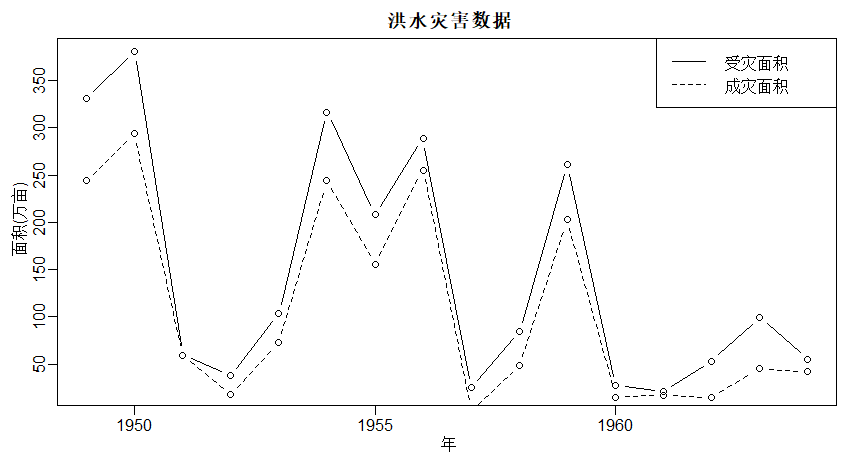
\includegraphics[width=0.7\textwidth]{1.png}
\end{figure}
\begin{lstlisting}[language=r]
> acf(xl)
\end{lstlisting}
\begin{figure}[H]
	\centering
	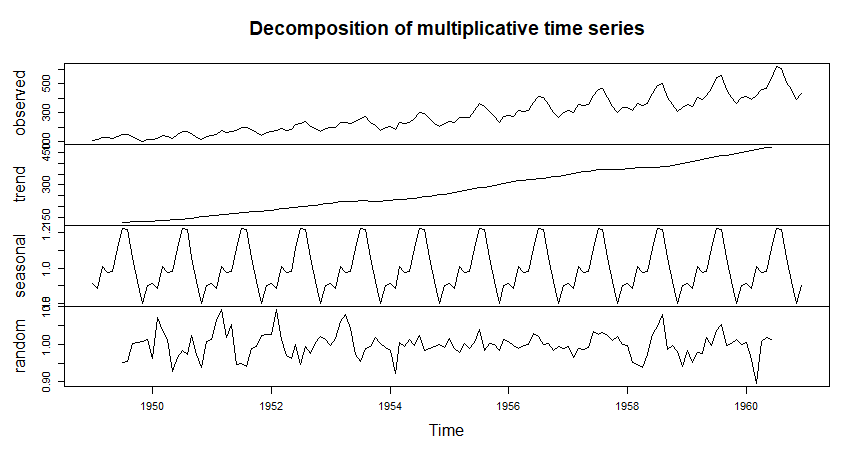
\includegraphics[width=0.7\textwidth]{11.png}
\end{figure}
\subsection{模型定阶和参数估计}
\begin{figure}[H]
	\centering
	\includegraphics[width=0.7\textwidth]{screenshot086}
	\label{fig:screenshot086}
\end{figure}
一般从高到低试p

\begin{lstlisting}[language=r]
> arima(t1,order=c(4,0,0),include.mean = T,method = "ML")

Call:
arima(x = t1, order = c(4, 0, 0), include.mean = T, method = "ML")

Coefficients:
         ar1      ar2     ar3      ar4
      1.5610  -1.2113  0.5189  -0.2472
s.e.  0.1364   0.2511  0.2555   0.1424
      intercept
        50.8131
s.e.     4.8898

sigma^2 estimated as 164.5:  log likelihood = -200.09,  aic = 412.18

\end{lstlisting}

参数检验和区间估计的函数:
\begin{lstlisting}[language=r]
t_test <- function(arma, alpha = 0.05){
	c <- arma$coef
	sd <- sqrt(diag(arma$var.coef)) 
	t <- abs(c/sd)
	k <- sum(arma$arma)
	n <- arma$nobs
	Pvalue <- 2*(1 - pt(t, df = n - k))
	t_alpha <- qt(1 - alpha/2, df = n - k)
	A <- rbind(c, c - t_alpha*sd, c + t_alpha*sd) 
	rownames(A) <- c("coef", "lwr", "upr")
	list(p_value = Pvalue, confint = A)
}

#函数自变量object是由arima()函数生成的对象
#alpha是显著性水平,默认值为0.05
#函数的返回值是列表,成员有p_value和confint,分别表示ARMA模型中参数检化验的p值和对应参数的置信区间.

\end{lstlisting}

误差度量:
\begin{lstlisting}[language=r]
> accuracy(at32)
                    ME     RMSE      MAE       MPE     MAPE     MASE
Training set -0.000552 0.035953 0.028222 -6.099606 20.15136 0.691440
                   ACF1
Training set 0.09337227
\end{lstlisting}
示例:
\begin{lstlisting}[language=r]
> at32<-arima(t32,order=c(4,0,0),include.mean = T,method = "ML")
> t_test(at32)
$p_value
         ar1          ar2          ar3          ar4    intercept 
1.783890e-06 5.767494e-03 3.450339e-02 1.872355e-02 1.276224e-11 

$confint
           ar1        ar2        ar3         ar4 intercept
coef 1.0446356 -0.7259678 0.52571027 -0.40687488 0.1470192
lwr  0.7004788 -1.2203376 0.04166464 -0.73987673 0.1217077
upr  1.3887924 -0.2315980 1.00975590 -0.07387304 0.1723308
\end{lstlisting}

\subsubsection{关于自动定阶:auto.arima()}
\begin{figure}[H]
	\centering
	\includegraphics[width=\textwidth]{screenshot087}
	\label{fig:screenshot087}
\end{figure}
\begin{figure}[H]
	\centering
	\includegraphics[width=\textwidth]{screenshot088}
	\label{fig:screenshot088}
\end{figure}
\begin{figure}[H]
	\centering
	\includegraphics[width=\textwidth]{screenshot089}
	\label{fig:screenshot089}
\end{figure}


\subsection{模型检验}

\subsubsection{残差的白噪声检验}
\begin{figure}[H]
	\includegraphics[width=0.85\textwidth]{screenshot020}
\end{figure}
\begin{lstlisting}[language=r]
> Box.test(at32$residuals,type = "Box-Pierce")

Box-Pierce test

data:  at32$residuals
X-squared = 0.25283, df = 1, p-value = 0.6151
\end{lstlisting}
\subsubsection{残差的正态性检验}
画出残差的QQ图即可判断,QQ图中残差基本完全落在45°线上即为符合正态性假设。否则模型可能出现错误。语法为:
\[qqnorm(model\$residuals)\]
\[qqline(model\$residuals)\]
\subsubsection{异方差检验}
\textbf{FinTS程序包的ArchTest函数}
\begin{lstlisting}[language=r]
> ArchTest(t1,lag=2)

ARCH LM-test; Null hypothesis: no ARCH effects

data:  t1
Chi-squared = 33.719, df = 2, p-value = 4.764e-08

> ArchTest(t1,lag=1)

ARCH LM-test; Null hypothesis: no ARCH effects

data:  t1
Chi-squared = 26.598, df = 1, p-value = 2.504e-07

# ARCH检验 原假设是存在异方差(存在ARCH效应)
\end{lstlisting}

\subsection{模型表达}

\subsection{预测}

\section{示例2}
\begin{lstlisting}[language=r]
> d1<-read.csv("E:/5.时间序列/机房eviews&R/时间序列数据_机房/表1.1.csv")
> t1<-ts(d1$heizishu,frequency = 1)
> plot(t1)
> library(fUnitRoots)
> adfTest(t1,lags = 1,type = "ct")

Title:
Augmented Dickey-Fuller Test

Test Results:
PARAMETER:
Lag Order: 1
STATISTIC:
Dickey-Fuller: -5.9831
P VALUE:
0.01 

Description:
Thu Dec 10 08:58:48 2020 by user: 14576

Warning message:
In adfTest(t1, lags = 1, type = "ct") :
p-value smaller than printed p-value
> adfTest(t1,lags = 1,type = "c")

Title:
Augmented Dickey-Fuller Test

Test Results:
PARAMETER:
Lag Order: 1
STATISTIC:
Dickey-Fuller: -5.9432
P VALUE:
0.01 

Description:
Thu Dec 10 08:59:45 2020 by user: 14576

Warning message:
In adfTest(t1, lags = 1, type = "c") : p-value smaller than printed p-value
> adfTest(t1,lags = 1,type = "nc")

Title:
Augmented Dickey-Fuller Test

Test Results:
PARAMETER:
Lag Order: 1
STATISTIC:
Dickey-Fuller: -2.3333
P VALUE:
0.02165 

Description:
Thu Dec 10 09:00:02 2020 by user: 14576
#故是带有常数项的平稳序列
#-----------------------------------------------------------
> acf(t1)
> pacf(t1)
#估为4阶q
#-----------------------------------------------------------
> arima(t1,order=c(4,0,0),include.mean = T,method = "ML")

Call:
arima(x = t1, order = c(4, 0, 0), include.mean = T, method = "ML")

Coefficients:
         ar1      ar2     ar3      ar4
      1.5610  -1.2113  0.5189  -0.2472
s.e.  0.1364   0.2511  0.2555   0.1424
      intercept
        50.8131
s.e.     4.8898

sigma^2 estimated as 164.5:  log likelihood = -200.09,  aic = 412.18

> arima(t1,order=c(3,0,0),include.mean = T,method = "ML")

Call:
arima(x = t1, order = c(3, 0, 0), include.mean = T, method = "ML")

Coefficients:
         ar1      ar2     ar3  intercept
      1.5319  -0.9786  0.1469    50.3086
s.e.  0.1393   0.2182  0.1433     6.2582

sigma^2 estimated as 175.2:  log likelihood = -201.54,  aic = 413.08

> arima(t1,order=c(2,0,0),include.mean = T,method = "ML")

Call:
arima(x = t1, order = c(2, 0, 0), include.mean = T, method = "ML")

Coefficients:
         ar1      ar2  intercept
      1.4208  -0.7728    50.6410
s.e.  0.0885   0.0874     5.4265

sigma^2 estimated as 179:  log likelihood = -202.06,  aic = 412.11

> arima(t1,order=c(1,0,0),include.mean = T,method = "ML")

Call:
arima(x = t1, order = c(1, 0, 0), include.mean = T, method = "ML")

Coefficients:
         ar1  intercept
      0.7954    48.0639
s.e.  0.0825    13.4874

sigma^2 estimated as 439.8:  log likelihood = -223.6,  aic = 453.21

#选p=2
#---------------------------------------------------------------------
> x1.fit<-arima(t1,order=c(2,0,0),include.mean = T,method = "ML")
> Box.test(x1.fit$residuals,lag = 6)

Box-Pierce test

data:  x1.fit$residuals
X-squared = 3.9931, df = 6, p-value = 0.6776

> Box.test(x1.fit$residuals,lag = 4)

Box-Pierce test

data:  x1.fit$residuals
X-squared = 2.8505, df = 4, p-value = 0.5831

#残差检验 原假设是不具有相关性  此处因此不拒绝原假设,通过了白噪声检验
#--------------------------------------------------------------------
> ArchTest(t1,lag=2)

ARCH LM-test; Null hypothesis: no ARCH effects

data:  t1
Chi-squared = 33.719, df = 2, p-value = 4.764e-08

> ArchTest(t1,lag=1)

ARCH LM-test; Null hypothesis: no ARCH effects

data:  t1
Chi-squared = 26.598, df = 1, p-value = 2.504e-07

# ARCh检验 原假设是不存在异方差
\end{lstlisting}
\begin{figure}[H]
	\centering
	\includegraphics[width=0.7\textwidth]{screenshot077}
	\label{fig:screenshot077}
\end{figure}

\begin{figure}[H]
	\centering
	\includegraphics[width=0.7\textwidth]{screenshot078}
	\label{fig:screenshot078}
\end{figure}
\section{示例3}
\begin{lstlisting}[language=r]
> d3<-read.csv("E:/5.时间序列/机房eviews&R/时间序列数据_机房/表1.3.csv")
> t3<-ts(d3$GDP,start=1978,frequency = 1)
> plot(t3)

> t31<-log(t3)
> plot(t31)
> t32<-diff(t31)
> plot(t32)

> adfTest(t32,lags = 1,type = "ct")

Title:
Augmented Dickey-Fuller Test

Test Results:
PARAMETER:
Lag Order: 1
STATISTIC:
Dickey-Fuller: -2.9936
P VALUE:
0.1917 

Description:
Thu Dec 10 10:05:53 2020 by user: 14576
> adfTest(t32,lags = 1,type = "c")

Title:
Augmented Dickey-Fuller Test

Test Results:
PARAMETER:
Lag Order: 1
STATISTIC:
Dickey-Fuller: -3.0437
P VALUE:
0.046 

Description:
Thu Dec 10 10:06:46 2020 by user: 14576

> adfTest(t1,lags = 1,type = "nc")

Title:
Augmented Dickey-Fuller Test

Test Results:
PARAMETER:
Lag Order: 1
STATISTIC:
Dickey-Fuller: -2.3333
P VALUE:
0.02165 

Description:
Thu Dec 10 10:10:18 2020 by user: 14576
> adfTest(t1,lags = 1,type = "nc")

Title:
Augmented Dickey-Fuller Test

Test Results:
PARAMETER:
Lag Order: 1
STATISTIC:
Dickey-Fuller: -2.3333
P VALUE:
0.02165 

Description:
Thu Dec 10 10:10:18 2020 by user: 14576

#含截距项平稳

> acf(t32)
> pacf(t32)
# p=4看看

> arima(t32,order=c(4,0,0),include.mean = T,method = "ML")

Call:
arima(x = t32, order = c(4, 0, 0), include.mean = T, method = "ML")

Coefficients:
         ar1      ar2     ar3      ar4  intercept
      1.0446  -0.7260  0.5257  -0.4069     0.1470
s.e.  0.1668   0.2395  0.2345   0.1613     0.0123

sigma^2 estimated as 0.001293:  log likelihood = 54.43,  aic = -96.85
> arima(t32,order=c(3,0,0),include.mean = T,method = "ML")

Call:
arima(x = t32, order = c(3, 0, 0), include.mean = T, method = "ML")

Coefficients:
         ar1      ar2     ar3  intercept
      0.9986  -0.4986  0.1047     0.1451
s.e.  0.1844   0.2437  0.1835     0.0184

sigma^2 estimated as 0.0016:  log likelihood = 51.69,  aic = -93.39
> arima(t32,order=c(2,0,0),include.mean = T,method = "ML")

Call:
arima(x = t32, order = c(2, 0, 0), include.mean = T, method = "ML")

Coefficients:
         ar1      ar2  intercept
      0.9513  -0.3947     0.1459
s.e.  0.1656   0.1633     0.0167

sigma^2 estimated as 0.00162:  log likelihood = 51.53,  aic = -95.07
> arima(t32,order=c(1,0,0),include.mean = T,method = "ML")

Call:
arima(x = t32, order = c(1, 0, 0), include.mean = T, method = "ML")

Coefficients:
         ar1  intercept
      0.6728     0.1445
s.e.  0.1299     0.0235

sigma^2 estimated as 0.001962:  log likelihood = 48.94,  aic = -91.88
\end{lstlisting}

\begin{figure}[H]
	\centering
	\includegraphics[width=0.7\textwidth]{screenshot079}
	\label{fig:screenshot079}
\end{figure}
\begin{figure}[H]
	\centering
	\includegraphics[width=0.7\textwidth]{screenshot080}
	\label{fig:screenshot080}
\end{figure}
\begin{figure}[H]
	\centering
	\includegraphics[width=0.7\textwidth]{screenshot081}
	\label{fig:screenshot081}
\end{figure}
\begin{figure}[H]
	\centering
	\includegraphics[width=0.7\textwidth]{screenshot082}
	\label{fig:screenshot082}
\end{figure}
\begin{figure}[H]
	\centering
	\includegraphics[width=0.7\textwidth]{screenshot083}
	\label{fig:screenshot083}
\end{figure}

%---------------------------------------------------------------------------------------%
\chapter{MA models}
\section{例子}
\begin{figure}[H]
	\centering
	\includegraphics[width=0.8\linewidth]{screenshot002}
	\label{fig:screenshot002}
\end{figure}
\begin{lstlisting}[language=r]
####3.2.2 MA models ####
#eg3-6
r1<-arima.sim(n=1000,list(ma=-2))
r2<-arima.sim(n=1000,list(ma=-0.5))
r3<-arima.sim(n=1000,list(ma=c(-0.8,16/25)))
r4<-arima.sim(n=1000,list(ma=c(-5/4,25/16)))
par(mfrow=c(4,2))
acf(r1)
acf(r2)
acf(r3)
acf(r4)
pacf(r1)
pacf(r2)
pacf(r3)
pacf(r4)
\end{lstlisting}
\begin{figure}[H]
	\centering
	\includegraphics[width=\linewidth]{screenshot001}
	\caption{}
	\label{fig:screenshot001}
\end{figure}
\section{几个重要的R函数(ldf 236)}
\subsection{从自协方差函数利用递推方法估计模型参数的函数}
\begin{lstlisting}[language=r]
## 从自协方差函数利用递推方法估计模型参数的函数
## Given \gamma_0, \gamma_1, \dots, \gamma_q,
## Solve MA(q) coefficients b_1, \dots, b_q, \sigma^2
## Using Li Lei's algorithm.
## Input: gms -- \gamma_0, \gamma_1, \dots, \gamma_q
ma.solve <- function(gms, k=100){
	q <- length(gms)-1
	if(q==1){
		rho1 <- gms[2] / gms[1]
		b <- (1 - sqrt(1 - 4*rho1^2))/(2*rho1)
		s2 <- gms[1] / (1 + b^2)
		return(list(b=b, s2=s2))
	}
	A <- matrix(0, nrow=q, ncol=q)
	for(j in seq(2,q)){
		A[j-1,j] <- 1
	}
	cc <- numeric(q); cc[1] <- 1
	gamma0 <- gms[1]
	gammas <- numeric(q+k)
	gammas[1:(q+1)] <- gms
	gamq <- gms[-1]
	Gammak <- matrix(0, nrow=k, ncol=k)
	for(ii in seq(k)){
		for(jj in seq(k)){
			Gammak[ii,jj] <- gammas[abs(ii-jj)+1]
		}
	}
	Omk <- matrix(0, nrow=q, ncol=k)
	for(ii in seq(q)){
		for(jj in seq(k)){
			Omk[ii,jj] <- gammas[ii+jj-1+1]
		}
	}
	PI <- Omk %*% solve(Gammak, t(Omk))
	s2 <- gamma0 - c(t(cc) %*% PI %*% cc)
	b <- 1/s2 * c(gamq - A %*% PI %*% cc)
	return(list(b=b, s2=s2))
}
\end{lstlisting}
\subsection{模拟MA 序列的函数}
\begin{lstlisting}[language=r]
## simulate MA(q) model.模拟MA 序列的函数
## a is vector a_1,..., a_q
## Model is X_t = eps_t + a_1 eps_{t-1} + ... + a_q eps_{t-q}
## \Var(\epsilon_t) = sigma^2
## This version uses the filter function.
ma.gen <- function(n, a, sigma=1.0, by.roots=FALSE,
plot.it=FALSE){
	if(by.roots){
		require(polynom)
		cf <- Re(c(poly.calc(a)))
		cf <- cf / cf[1]
		a <- cf
	}
	q <- length(a)
	n2 <- n+q
	eps <- rnorm(n2, 0, sigma)
	x2 <- filter(eps, c(1,a), method="convolution", side=1)
	x <- x2[(q+1):n2]
	x <- ts(x)
	attr(x, "model") <- "MA"
	attr(x, "b") <- a
	attr(x, "sigma") <- sigma
	if(plot.it) plot(x)
	x
}
\end{lstlisting}
\subsection{绘制MA 理论谱密度曲线的函数}
\begin{lstlisting}[language=r]
## MA theoretical spectrum given MA coefficients
## 绘制MA 理论谱密度曲线的函数
ma.true.spectrum <- function(a, ngrid=256, sigma=1,
tit="True MA Spectral Density",
plot.it=TRUE){
	p <- length(a)
	freqs <- seq(from=0, to=pi, length=ngrid)
	spec <- numeric(ngrid)
	for(ii in seq(ngrid)){
		spec[ii] <- 1 + sum(complex(mod=a, arg=freqs[ii]*seq(p)))
	}
	spec = sigma^2 / (2*pi) * abs(spec)^2
	if(plot.it){
		plot(freqs, spec, type='l',
		main=tit,
		xlab="frequency", ylab="spectrum",
		axes=FALSE)
		axis(2)
		axis(1, at=(0:6)/6*pi,
		labels=c(0, expression(pi/6),
		expression(pi/3), expression(pi/2),
		expression(2*pi/3), expression(5*pi/6), expression(pi)))
		box()
	}
	invisible(list(frequencies=freqs, spectrum=spec,
	ma.coefficients=a, sigma=sigma))
}
\end{lstlisting}
%----------------------------------------------------------------------------------------%
\chapter{ARMA models}
\begin{figure}[H]
	\centering
	\includegraphics[width=0.8\linewidth]{screenshot003}
	\caption{}
	\label{fig:screenshot003}
\end{figure}

\begin{lstlisting}[language=r]
####3.2.3 ARMA models ####
#eg3-8
t<-arima.sim(n=1000,list(ar=0.5,ma=-0.8))
acf(t)
pacf(t)
\end{lstlisting}
\section{几个R函数}
\subsection{给定ARMA系数的ARMA理论谱}
\begin{lstlisting}[language=r]
## ARMA theoretical spectrum given ARMA coefficients
arma.true.spectrum <- function(a, b, ngrid=256, sigma=1,
tit="True ARMA Spectral Density",
plot.it=TRUE){
	p <- length(a)
	q <- length(b)
	freqs <- seq(from=0, to=pi, length=ngrid)
	spec1 <- numeric(ngrid)
	spec2 <- numeric(ngrid)
	for(ii in seq(ngrid)){
		spec1[ii] <- 1 + sum(complex(mod=b, arg=freqs[ii]*seq(q)))
		spec2[ii] <- 1 - sum(complex(mod=a, arg=freqs[ii]*seq(p)))
	}
	spec = sigma^2 / (2*pi) * abs(spec1)^2 / abs(spec2)^2
	if(plot.it){
		plot(freqs, spec, type='l',
		main=tit,
		xlab="frequency", ylab="spectrum",
		axes=FALSE)
		axis(2)
		axis(1, at=(0:6)/6*pi,
		labels=c(0, expression(pi/6),
		expression(pi/3), expression(pi/2),
		expression(2*pi/3), expression(5*pi/6), expression(pi)))
	}
	box()
	invisible(list(frequencies=freqs, spectrum=spec,
	ar.coefficients=a, ma.coefficients=b,
	sigma=sigma))
}
\end{lstlisting}
\subsection{模拟ARMA(p, q)模型}
\begin{lstlisting}[language=r]
## simulate ARMA(p, q) model.
## a is vector a_1, \dots, a_p
## b is vector b_1, \dots, b_q
## Model is
## X_t = a_1 X_{t-1} + \dots + a_p X_{t-p}
## + \epsilon_t + b_1 \epsilon_{t-1} + \dots + b_q \epsilon_{t-q}
## \Var(\epsilon_t) = sigma^2
arma.gen <- function(n, a, b, sigma=1.0,
by.roots.ar=FALSE, by.roots.ma=FALSE,
plot.it=FALSE, n0=1000,
x0=numeric(length(a))){
	n2 <- n0 + n
	p <- length(a)
	## first generate n0+n MA(q) series
	eps <- ma.gen(n2, b, sigma=sigma,
	by.roots=by.roots.ma,
	plot.it=FALSE)
	b <- attr(eps, "b")
	if(by.roots.ar){
		require(polynom)
		cf <- Re(c(poly.calc(a)))
		cf <- cf / cf[1]
		a <- -cf[-1]
	}
	##set.seed(1)
	x2 <- filter(eps, a, method="recursive", side=1, init=x0)
	x <- x2[(n0+1):n2]
	x <- ts(x)
	attr(x, "model") <- "ARMA"
	attr(x, "a") <- a
	attr(x, "b") <- b
	attr(x, "sigma") <- sigma
	if(plot.it) plot(x)
	x
}
\end{lstlisting}
\subsection{ARMA模型的Wold系数}
\begin{lstlisting}[language=r]
## Wold coefficients for the ARMA model
arma.Wold <- function(n, a, b=numeric(0)){
	p <- length(a)
	q <- length(b)
	arev <- rev(a)
	psi <- numeric(n)
	psi[1] <- 1
	for(j in seq(n-1)){
		if(j <= q) bj=b[j]
		else bj=0
		psis <- psi[max(1, j+1-p):j]
		np <- length(psis)
		if(np < p) psis <- c(rep(0,p-np), psis)
		psi[j+1] <- bj + sum(arev * psis)
	}
	psi
}
\end{lstlisting}
\subsection{利用Wold展开计算ARMA模型的理论自协方差函数}
\begin{lstlisting}[language=r]
## Calculate theoretical autocovariance function
## of ARMA model using Wold expansion
arma.gamma.by.Wold <- function(n, a, b=numeric(0), sigma=1){
	nn <- n + 100
	psi <- arma.Wold(nn, a, b)
	gam <- numeric(n)
	for(ii in seq(0, n-1)){
		gam[ii+1] <- sum(psi[1:(nn-ii)] * psi[(ii+1):nn])
	}
	gam <- (sigma^2) * gam
	gam
}
arma.gamma <- arma.gamma.by.Wold
\end{lstlisting}
\subsection{求解给定自协方差函数的ARMA参数}
\begin{lstlisting}[language=r]
## Solve ARMA parameters given autocovariance functions
arma.solve <- function(gms, p, q){
	Gpq <- matrix(0, nrow=p, ncol=p)
	for(ii in seq(p)) for(jj in seq(p)){
		Gpq[ii,jj] <- gms[abs(q + ii - jj)+1]
	}
	gs <- gms[(q+1+1):(q+p+1)]
	a <- solve(Gpq, gs)
	aa <- c(-1, a)
	gys <- numeric(q+1)
	for(k in seq(0, q)){
		gys[k+1] <- sum(c(outer(0:p,0:p,
		function(ii,jj) aa[ii+1] * aa[jj+1]
		* gms[abs(k+jj-ii)+1])))
	}
	res <- ma.solve(gys)
	b <- res$b
	sigma <- sqrt(res$s2)
	list(a=a, b=b, sigma=sigma)
}
\end{lstlisting}
%-----------------------------------------------------------------------------------------%
\chapter{建模}
\begin{lstlisting}[language=r]
#### 建模 ####
library(zoo)
library(forecast)
auto.arima(bwi)
\end{lstlisting}


%-----------------------------------------------------------------------------------------%
\part{多元时间序列分析}
\chapter{单位根检验}
\begin{figure}[H]
	\includegraphics[width=0.85\textwidth]{screenshot022}
	\label{fig:screenshot022}
\end{figure}

\section{DF检验}
\subsection{DF统计量}
\begin{figure}[H]
	\includegraphics[width=0.85\textwidth]{screenshot023}
	\label{fig:screenshot023}
\end{figure}
\begin{figure}[H]
	\includegraphics[width=0.85\textwidth]{screenshot024}
	\label{fig:screenshot024}
\end{figure}
\begin{figure}[H]
	\includegraphics[width=0.85\textwidth]{screenshot025}
	\label{fig:screenshot025}
\end{figure}
\begin{figure}[H]
	\includegraphics[width=0.85\textwidth]{screenshot026}
	\label{fig:screenshot026}
\end{figure}
\begin{figure}[H]
	\includegraphics[width=0.85\textwidth]{screenshot027}
	\label{fig:screenshot027}
\end{figure}
\begin{figure}[H]
	\includegraphics[width=0.85\textwidth]{screenshot028}
	\label{fig:screenshot028}
\end{figure}
\subsection{DF检验的等价表达}
\begin{figure}[H]
	\includegraphics[width=0.85\textwidth]{screenshot029}
	\label{fig:screenshot029}
\end{figure}
\subsection{DF检验的三种类型}
因为非平稳的构成很复杂,不同结构的非平稳序列选择的分析方法也不同.通常把非平稳分成三大类.
\subsubsection{无漂移项自回归过程}
\begin{figure}[H]
	\includegraphics[width=0.85\textwidth]{screenshot030}
	\label{fig:screenshot030}
\end{figure}
\subsubsection{带漂移项自回归过程}
\begin{figure}[H]
	\includegraphics[width=0.85\textwidth]{screenshot031}
	\label{fig:screenshot031}
\end{figure}
\begin{figure}[H]
	\includegraphics[width=0.85\textwidth]{screenshot032}
	\label{fig:screenshot032}
\end{figure}
\begin{figure}[H]
	\includegraphics[width=0.85\textwidth]{screenshot033}
	\label{fig:screenshot033}
\end{figure}
\begin{lstlisting}[language=r]
> e<-rnorm(1000)
'arg' should be one of “convolution”, “recursive”
> x<-filter(0.1+e,filter=1,method="recursive") #拟合带漂移项的自回归过程
> plot(x)

> t<-c(1:1000)
> abline(lm(x~t),col=2)
> lm(x~t)

Call:
lm(formula = x ~ t)

Coefficients:
(Intercept)            t  
    -1.9701       0.1101  
\end{lstlisting}
\begin{figure}[H]
	\includegraphics[width=\textwidth]{screenshot034}
	\label{fig:screenshot034}
\end{figure}
\begin{figure}[H]
	\includegraphics[width=0.85\textwidth]{screenshot035}
	\label{fig:screenshot035}
\end{figure}

\begin{tcolorbox}[colback=pink!10!white,colframe=pink!100!black]
	\textbf{filter(x, filter, method = c("convolution", "recursive"), sides = 2, circular = FALSE, init)}
	\begin{itemize}
		\item x: 一元或多元时间序列。
		\item filter: 一个反向的时间顺序滤波器系数向量(AR或MA系数)。
		\item method: "convolution"或者"recursive"(可以缩写),如果是"convolution"则是移动平均,如果是"recursive"则是自回归。
		\item sides: 卷积过滤器。如果sides=1滤波器系数是对过去的价值观;如果sides=2他们周围滞后0为中心的。在这种情况下,过滤器的长度应为奇数,但如果它是偶数,过滤器的更多的是向前的时间比落后。
		\item circular: 卷积过滤器。如果TRUE,包装左右两端系列的过滤,否则假定缺少外部值(NA)。
		\item init: 只有递归滤波器。指定的时间序列的初始值,只是之前的起始值,反向时间顺序。默认的是一套零。
	\end{itemize}
\end{tcolorbox}

差分运算和线性拟合后的残差比较
\begin{lstlisting}[language=r]
> r1<-diff(x)
> x.fit<-lm(x~t)
> r2<-ts(x.fit$residuals)
> c1<-min(r1,r2)
> c2<-max(r1,r2)
> plot(r1,ylim=c(c1,c2))
> lines(r2,col=2)
\end{lstlisting}
\begin{figure}[H]
	\includegraphics[width=\textwidth]{screenshot036}
	\label{fig:screenshot036}
\end{figure}

\subsubsection{带趋势项回归过程}
\begin{figure}[H]
	\includegraphics[width=0.85\textwidth]{screenshot037}
	\label{fig:screenshot037}
\end{figure}
\begin{figure}[H]
	\includegraphics[width=0.85\textwidth]{screenshot038}
	\label{fig:screenshot038}
\end{figure}

\begin{lstlisting}[language=r]
> t<-c(1:1000)
> e<-rnorm(1000,0,10)
> x<-0.1*t+e
> x<-ts(x)
> plot(x)
\end{lstlisting}
\begin{figure}[H]
	\includegraphics[width=\textwidth]{screenshot039}
	\label{fig:screenshot039}
\end{figure}

考察差分后残差序列的波动范围:
\begin{lstlisting}[language=r]
> plot(diff(x))
> abline(h=c(1.98*sd(diff(x)),-1.98*sd(diff(x))),col=2)
\end{lstlisting}
\begin{figure}[H]
	\includegraphics[width=\textwidth]{screenshot041}
	\label{fig:screenshot041}
\end{figure}

图中两条平行线为该残差序列的95\%置信区间.

考察线性拟合后残差序列的波动范围
\begin{lstlisting}[language=r]
> x.fit<-lm(x~t)
> r<-ts(x.fit$residuals)
> plot(r)
> abline(h=c(1.98*sd(r),-1.98*sd(r)),col=2)
\end{lstlisting}
\begin{figure}[H]
	\includegraphics[width=\textwidth]{screenshot042}
	\label{fig:screenshot042}
\end{figure}
\begin{figure}[H]
	\includegraphics[width=0.85\textwidth]{screenshot043}
	\label{fig:screenshot043}
\end{figure}

\subsection{DF检验}
\begin{figure}[H]
	\includegraphics[width=0.85\textwidth]{screenshot044}
	\label{fig:screenshot044}
\end{figure}

\begin{lstlisting}[language=r]
> library(fUnitRoots)
载入需要的程辑包:timeDate
载入需要的程辑包:timeSeries
载入需要的程辑包:fBasics
> bj<-read.csv("E:/5.时间序列/机房eviews&R/时间序列数据_机房/表1.13.csv")
> lnbj<-log(bj$收入)
> x<-ts(lnbj)
> plot(x)


> adfTest(x,lag=1,type="nc") #=============================

Title:
Augmented Dickey-Fuller Test

Test Results:
PARAMETER:
Lag Order: 1
STATISTIC:
Dickey-Fuller: 7.8053
P VALUE:
0.99 

Description:
Mon Dec 07 20:21:18 2020 by user: 14576

Warning message:
In adfTest(x, lag = 1, type = "nc") : p-value greater than printed p-value


> adfTest(x,lag=1,type="c") #=============================

Title:
Augmented Dickey-Fuller Test

Test Results:
PARAMETER:
Lag Order: 1
STATISTIC:
Dickey-Fuller: 4.3165
P VALUE:
0.99 

Description:
Mon Dec 07 20:21:56 2020 by user: 14576

Warning message:
In adfTest(x, lag = 1, type = "c") : p-value greater than printed p-value


> adfTest(x,lag=1,type="ct") #=============================

Title:
Augmented Dickey-Fuller Test

Test Results:
PARAMETER:
Lag Order: 1
STATISTIC:
Dickey-Fuller: 1.2591
P VALUE:
0.99 

Description:
Mon Dec 07 20:22:01 2020 by user: 14576

Warning message:
In adfTest(x, lag = 1, type = "ct") : p-value greater than printed p-value
\end{lstlisting}
\begin{figure}[H]
	\includegraphics[width=\textwidth]{screenshot045}
	\label{fig:screenshot045}
\end{figure}
在显著性水平取0.05时,可认为该序列为非平稳序列,这与时序图的表现一致.

\section{ADF检验}
\begin{figure}[H]
	\includegraphics[width=0.85\textwidth]{screenshot046}
	\label{fig:screenshot046}
\end{figure}
\subsection{ADF检验的原理}
\begin{figure}[H]
	\includegraphics[width=0.85\textwidth]{screenshot047}
	\label{fig:screenshot047}
\end{figure}
\begin{figure}[H]
	\includegraphics[width=0.85\textwidth]{screenshot048}
	\label{fig:screenshot048}
\end{figure}
\begin{figure}[H]
	\includegraphics[width=0.85\textwidth]{screenshot049}
	\label{fig:screenshot049}
\end{figure}
\begin{figure}[H]
	\includegraphics[width=0.85\textwidth]{screenshot050}
	\label{fig:screenshot050}
\end{figure}
\subsection{ADF检验的三种类型}
\begin{lstlisting}[language=r]
	
\end{lstlisting}
\begin{lstlisting}[language=r]
	
\end{lstlisting}
\begin{lstlisting}[language=r]
	
\end{lstlisting}
\begin{lstlisting}[language=r]
	
\end{lstlisting}
\begin{lstlisting}[language=r]
	
\end{lstlisting}
\begin{lstlisting}[language=r]
	
\end{lstlisting}
\begin{lstlisting}[language=r]
	
\end{lstlisting}
\begin{lstlisting}[language=r]
	
\end{lstlisting}
\begin{lstlisting}[language=r]
	
\end{lstlisting}
\begin{lstlisting}[language=r]
	
\end{lstlisting}
\begin{lstlisting}[language=r]
	
\end{lstlisting}
\begin{lstlisting}[language=r]
	
\end{lstlisting}
\begin{lstlisting}[language=r]
	
\end{lstlisting}
\begin{lstlisting}[language=r]
	
\end{lstlisting}
\begin{lstlisting}[language=r]
	
\end{lstlisting}
\begin{lstlisting}[language=r]
	
\end{lstlisting}
\begin{lstlisting}[language=r]
	
\end{lstlisting}
\begin{lstlisting}[language=r]
	
\end{lstlisting}
\begin{lstlisting}[language=r]
	
\end{lstlisting}
\begin{lstlisting}[language=r]
	
\end{lstlisting}
\begin{lstlisting}[language=r]
	
\end{lstlisting}


\end{document}